% Options for packages loaded elsewhere
\PassOptionsToPackage{unicode}{hyperref}
\PassOptionsToPackage{hyphens}{url}
\PassOptionsToPackage{dvipsnames,svgnames,x11names}{xcolor}
%
\documentclass[
  letterpaper,
  DIV=11,
  numbers=noendperiod]{scrartcl}

\usepackage{amsmath,amssymb}
\usepackage{lmodern}
\usepackage{iftex}
\ifPDFTeX
  \usepackage[T1]{fontenc}
  \usepackage[utf8]{inputenc}
  \usepackage{textcomp} % provide euro and other symbols
\else % if luatex or xetex
  \usepackage{unicode-math}
  \defaultfontfeatures{Scale=MatchLowercase}
  \defaultfontfeatures[\rmfamily]{Ligatures=TeX,Scale=1}
\fi
% Use upquote if available, for straight quotes in verbatim environments
\IfFileExists{upquote.sty}{\usepackage{upquote}}{}
\IfFileExists{microtype.sty}{% use microtype if available
  \usepackage[]{microtype}
  \UseMicrotypeSet[protrusion]{basicmath} % disable protrusion for tt fonts
}{}
\makeatletter
\@ifundefined{KOMAClassName}{% if non-KOMA class
  \IfFileExists{parskip.sty}{%
    \usepackage{parskip}
  }{% else
    \setlength{\parindent}{0pt}
    \setlength{\parskip}{6pt plus 2pt minus 1pt}}
}{% if KOMA class
  \KOMAoptions{parskip=half}}
\makeatother
\usepackage{xcolor}
\setlength{\emergencystretch}{3em} % prevent overfull lines
\setcounter{secnumdepth}{-\maxdimen} % remove section numbering
% Make \paragraph and \subparagraph free-standing
\ifx\paragraph\undefined\else
  \let\oldparagraph\paragraph
  \renewcommand{\paragraph}[1]{\oldparagraph{#1}\mbox{}}
\fi
\ifx\subparagraph\undefined\else
  \let\oldsubparagraph\subparagraph
  \renewcommand{\subparagraph}[1]{\oldsubparagraph{#1}\mbox{}}
\fi


\providecommand{\tightlist}{%
  \setlength{\itemsep}{0pt}\setlength{\parskip}{0pt}}\usepackage{longtable,booktabs,array}
\usepackage{calc} % for calculating minipage widths
% Correct order of tables after \paragraph or \subparagraph
\usepackage{etoolbox}
\makeatletter
\patchcmd\longtable{\par}{\if@noskipsec\mbox{}\fi\par}{}{}
\makeatother
% Allow footnotes in longtable head/foot
\IfFileExists{footnotehyper.sty}{\usepackage{footnotehyper}}{\usepackage{footnote}}
\makesavenoteenv{longtable}
\usepackage{graphicx}
\makeatletter
\def\maxwidth{\ifdim\Gin@nat@width>\linewidth\linewidth\else\Gin@nat@width\fi}
\def\maxheight{\ifdim\Gin@nat@height>\textheight\textheight\else\Gin@nat@height\fi}
\makeatother
% Scale images if necessary, so that they will not overflow the page
% margins by default, and it is still possible to overwrite the defaults
% using explicit options in \includegraphics[width, height, ...]{}
\setkeys{Gin}{width=\maxwidth,height=\maxheight,keepaspectratio}
% Set default figure placement to htbp
\makeatletter
\def\fps@figure{htbp}
\makeatother

\KOMAoption{captions}{tableheading}
\makeatletter
\makeatother
\makeatletter
\makeatother
\makeatletter
\@ifpackageloaded{caption}{}{\usepackage{caption}}
\AtBeginDocument{%
\ifdefined\contentsname
  \renewcommand*\contentsname{Table of contents}
\else
  \newcommand\contentsname{Table of contents}
\fi
\ifdefined\listfigurename
  \renewcommand*\listfigurename{List of Figures}
\else
  \newcommand\listfigurename{List of Figures}
\fi
\ifdefined\listtablename
  \renewcommand*\listtablename{List of Tables}
\else
  \newcommand\listtablename{List of Tables}
\fi
\ifdefined\figurename
  \renewcommand*\figurename{Figure}
\else
  \newcommand\figurename{Figure}
\fi
\ifdefined\tablename
  \renewcommand*\tablename{Table}
\else
  \newcommand\tablename{Table}
\fi
}
\@ifpackageloaded{float}{}{\usepackage{float}}
\floatstyle{ruled}
\@ifundefined{c@chapter}{\newfloat{codelisting}{h}{lop}}{\newfloat{codelisting}{h}{lop}[chapter]}
\floatname{codelisting}{Listing}
\newcommand*\listoflistings{\listof{codelisting}{List of Listings}}
\makeatother
\makeatletter
\@ifpackageloaded{caption}{}{\usepackage{caption}}
\@ifpackageloaded{subcaption}{}{\usepackage{subcaption}}
\makeatother
\makeatletter
\@ifpackageloaded{tcolorbox}{}{\usepackage[many]{tcolorbox}}
\makeatother
\makeatletter
\@ifundefined{shadecolor}{\definecolor{shadecolor}{rgb}{.97, .97, .97}}
\makeatother
\makeatletter
\makeatother
\ifLuaTeX
  \usepackage{selnolig}  % disable illegal ligatures
\fi
\IfFileExists{bookmark.sty}{\usepackage{bookmark}}{\usepackage{hyperref}}
\IfFileExists{xurl.sty}{\usepackage{xurl}}{} % add URL line breaks if available
\urlstyle{same} % disable monospaced font for URLs
\hypersetup{
  pdftitle={Optimization of solid waste in Blantyre, Malawi},
  pdfauthor={Nicolas Seemann-Ricard},
  colorlinks=true,
  linkcolor={blue},
  filecolor={Maroon},
  citecolor={Blue},
  urlcolor={Blue},
  pdfcreator={LaTeX via pandoc}}

\title{Optimization of solid waste in Blantyre, Malawi}
\author{Nicolas Seemann-Ricard}
\date{}

\begin{document}
\maketitle
\ifdefined\Shaded\renewenvironment{Shaded}{\begin{tcolorbox}[breakable, frame hidden, interior hidden, sharp corners, boxrule=0pt, enhanced, borderline west={3pt}{0pt}{shadecolor}]}{\end{tcolorbox}}\fi

\hypertarget{abstract}{%
\section{Abstract}\label{abstract}}

\hypertarget{introduction}{%
\section{Introduction}\label{introduction}}

The project seeks to minimize the costs of operation of the municipal
solid waste management service in Blantyre Malawi.

\hypertarget{justification-and-research-questions}{%
\subsection{Justification and Research
Questions}\label{justification-and-research-questions}}

\begin{enumerate}
\def\labelenumi{\arabic{enumi}.}
\tightlist
\item
  How can we model with limited data
\item
  How many trucks are needed to service all skips? What would be the
  mileage and cost of servicing all skips without overflow?
\item
  What routing schedule?
\end{enumerate}

\hypertarget{data-analysis}{%
\section{Data analysis}\label{data-analysis}}

In order to formulate feasible and pertinent recommendations, parameters
reflecting the situation need to be calculated. Specifically, the rate
at which bins are filling, so as to know the frequency at which they
need to be emptied.

\hypertarget{provided-data}{%
\subsection{Provided data}\label{provided-data}}

\hypertarget{set-of-skips}{%
\subsubsection{Set of skips}\label{set-of-skips}}

\hypertarget{skips-filling-data}{%
\subsubsection{Skips filling data}\label{skips-filling-data}}

Filling data for a number of skips is provided. Over a certain period of
time (depending on the skip), a measurement on a scale from 1-5 was
taken visually every day (generally). A score between 0 and 4 indicate
the estimated fullness of the skip, while a 5 means the skip was
overflowing. Three of these are shown below: alsdkjf

\begin{figure}

\begin{minipage}[t]{0.50\linewidth}

{\centering 

\raisebox{-\height}{

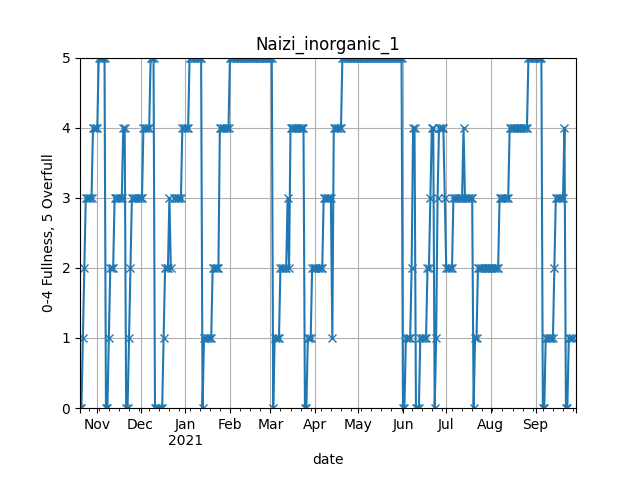
\includegraphics{../../src/Analysis_jupyter/figures/raw/Naizi_inorganic_1_raw.png}

}

}

\subcaption{\label{fig-Naizi_inorganic_1_raw}Naizi inorganic 1}
\end{minipage}%
%
\begin{minipage}[t]{0.50\linewidth}

{\centering 

\raisebox{-\height}{

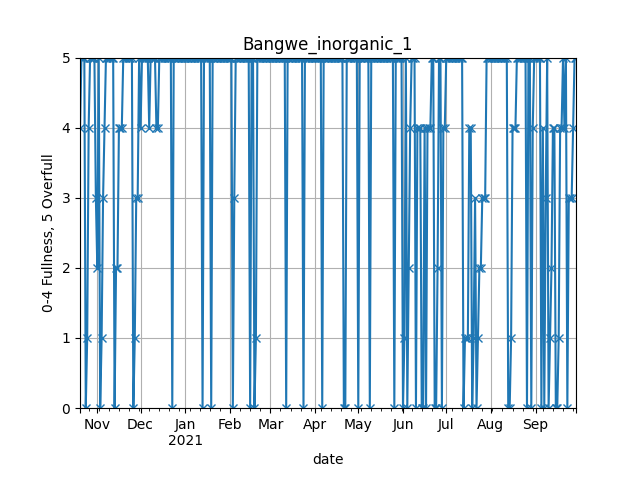
\includegraphics{../../src/Analysis_jupyter/figures/raw/Bangwe_inorganic_1_raw.png}

}

}

\subcaption{\label{fig-Bangwe_inorganic_1_raw}Bangwe inorganic 1}
\end{minipage}%
\newline
\begin{minipage}[t]{0.50\linewidth}

{\centering 

\raisebox{-\height}{

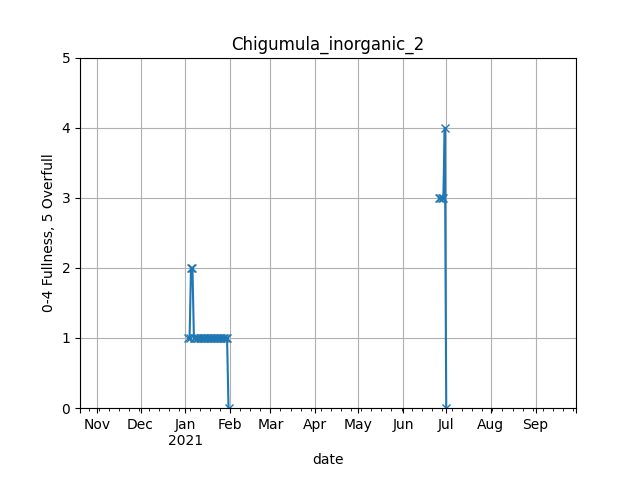
\includegraphics{../../src/Analysis_jupyter/figures/raw/Chigumula_inorganic_2_raw.png}

}

}

\subcaption{\label{fig-Chigumula_inorganic_2_raw}Chigumula inorganic 2}
\end{minipage}%
%
\begin{minipage}[t]{0.50\linewidth}

{\centering 

\raisebox{-\height}{

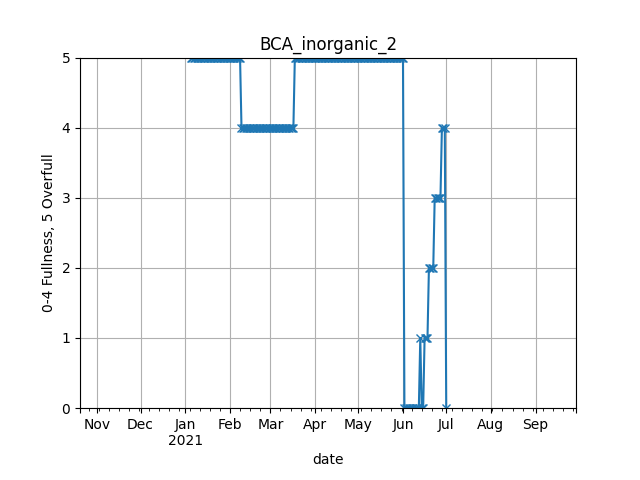
\includegraphics{../../src/Analysis_jupyter/figures/raw/BCA_inorganic_2_raw.png}

}

}

\subcaption{\label{fig-BCA_inorganic_2_raw}BCA inorganic 2}
\end{minipage}%

\caption{\label{fig-raw}Types of raw data}

\end{figure}

Fig.~\ref{fig-raw} is good, especially
fig.~\ref{fig-BCA_inorganic_2_raw}

\hypertarget{mzedi-arrivals}{%
\subsubsection{Mzedi arrivals}\label{mzedi-arrivals}}

\hypertarget{model}{%
\section{Model}\label{model}}

\hypertarget{model-optimization}{%
\section{Model optimization}\label{model-optimization}}

\hypertarget{methods}{%
\section{Methods}\label{methods}}

\hypertarget{site-selection}{%
\subsection{Site selection}\label{site-selection}}

\hypertarget{sample-size}{%
\subsection{Sample Size}\label{sample-size}}

\hypertarget{ethics}{%
\subsection{Ethics}\label{ethics}}

\hypertarget{experimental-design}{%
\subsection{Experimental Design}\label{experimental-design}}

\hypertarget{experiment-1}{%
\subsubsection{Experiment 1}\label{experiment-1}}

\hypertarget{experiment-2}{%
\subsubsection{Experiment 2}\label{experiment-2}}

\hypertarget{results-and-discussion}{%
\section{Results and Discussion}\label{results-and-discussion}}

\hypertarget{discussion}{%
\subsection{Discussion}\label{discussion}}

\hypertarget{tables-and-figures}{%
\subsection{Tables and Figures}\label{tables-and-figures}}

\hypertarget{tables}{%
\subsection{Tables}\label{tables}}

\hypertarget{figures}{%
\subsection{Figures}\label{figures}}

\hypertarget{conclusions-and-recommendations}{%
\section{Conclusions and
Recommendations}\label{conclusions-and-recommendations}}

\hypertarget{references}{%
\section{References}\label{references}}



\end{document}
